\documentclass[12pt]{article}
\usepackage[utf8]{inputenc}
\usepackage[T1]{fontenc}
\usepackage{geometry}
\usepackage{graphicx}
\usepackage{makeidx}
\geometry{margin=2.5cm}
\usepackage{fancyhdr}

\begin{document}
	
    \thispagestyle{empty}
	
    \begin{center}
        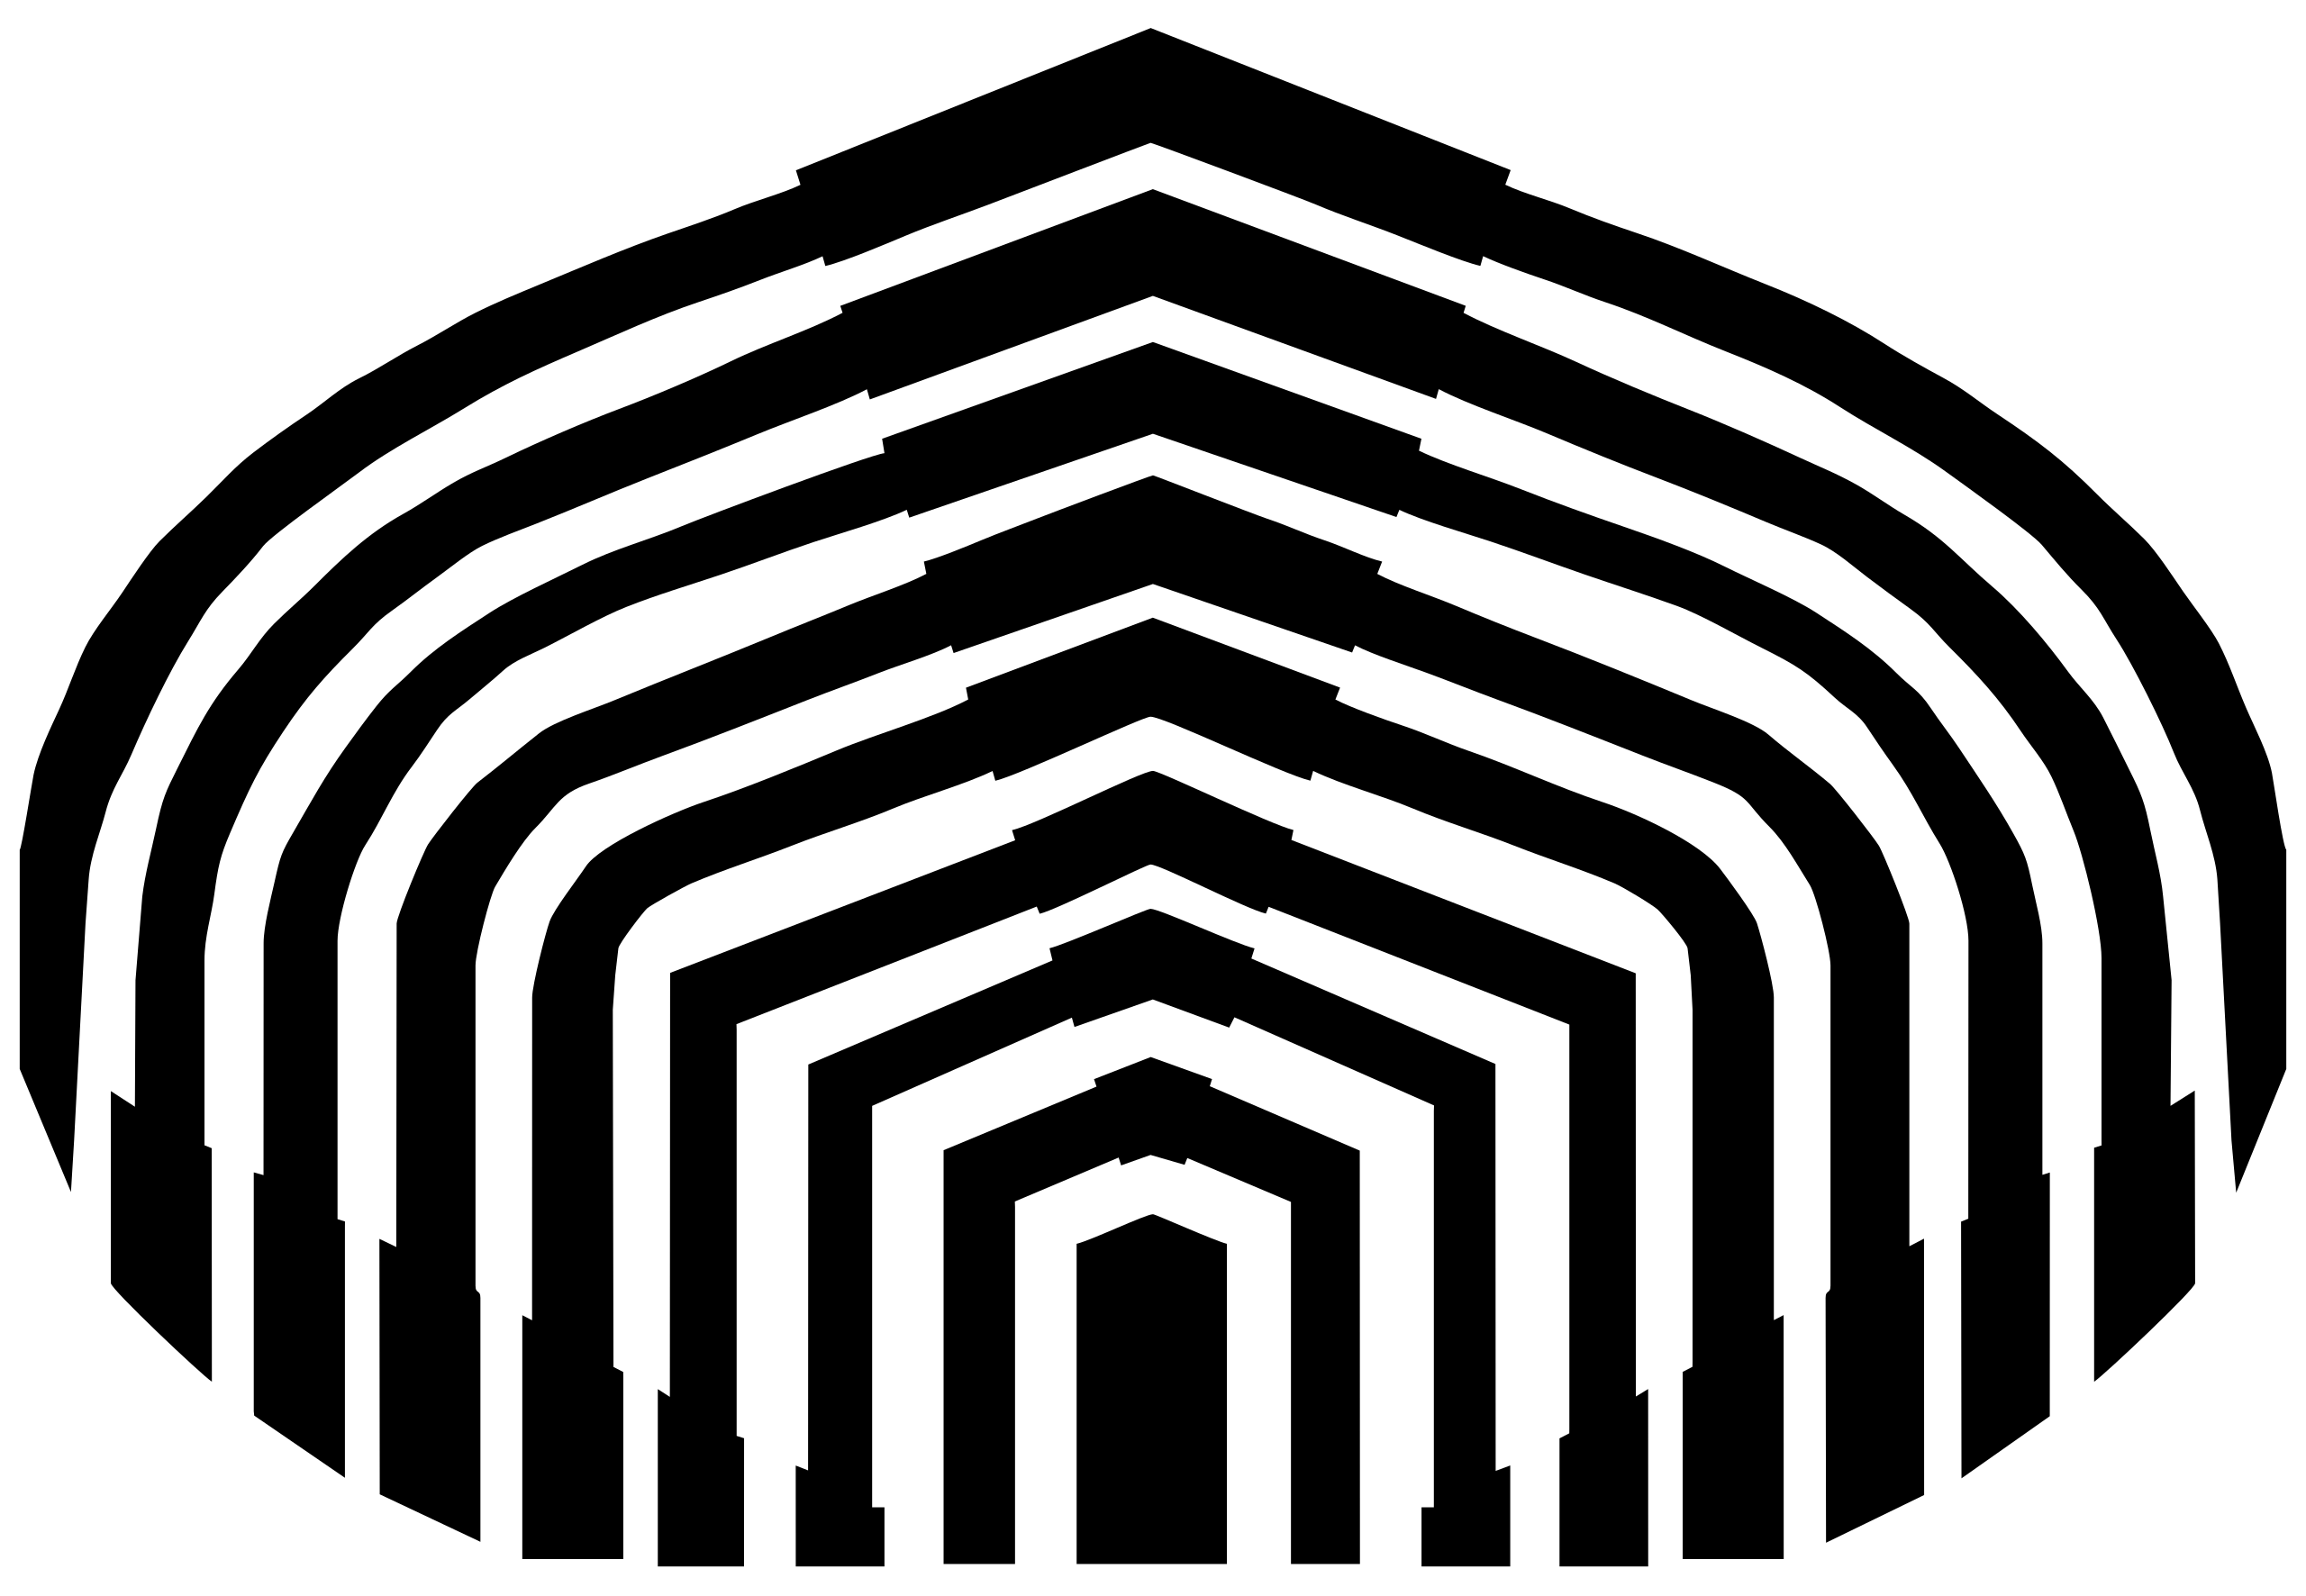
\includegraphics[width=3.1cm,height=2cm]{logo}\\
        UNIVERSIDAD SIMÓN BOLÍVAR\\
        DEPARTAMENTO DE ELECTRÓNICA Y CIRCUITOS\\
        EC1281 - LABORATORIO DE MEDICIONES ELÉCTRICAS\\
        SECCIÓN 1 - GRUPO 1\\
        
        \vspace{7cm}
        \textbf{\Large INFORME - PRÁCTICA \#6}\\
        MEDICIONES EN AC CON EL OSCILOSCOPIO CIRCUITO RLC SERIE\\
    \end{center}
    
    \begin{flushleft}
        \vspace{9cm}
        \hfill Integrantes:\\
        \hfill {\large Luis Becerra - 1910557}\\
        \hfill {\large Lorena Rojas - 1910469}\\
    \end{flushleft}
    
    \newpage
    
    \pagenumbering{Roman}
        \setcounter{page}{2}
    
    \begin{center}
        \textbf{\large RESUMEN}\\
    \end{center}
	
    En este informe de laboratorio de mediciones eléctricas, el objetivo fue utilizar el osciloscopio para observar formas de onda, medir amplitudes, frecuencias y desfasajes de señales eléctricas, así como estudiar las respuestas al escalón de circuitos RLC serie y analizar la respuesta en frecuencia de un circuito RLC serie utilizado como filtro pasabanda, elimina-banda, pasa-bajo y pasa-alto. El procedimiento consistió en montar y ajustar los circuitos, realizar mediciones en el osciloscopio y registrar los valores correspondientes. Los resultados más relevantes incluyeron la identificación de los tipos de respuesta de los circuitos RLC, la determinación de la frecuencia de resonancia, frecuencias de corte, ancho de banda y factor de calidad. Las conclusiones fundamentales indicaron que los circuitos RLC presentan diferentes comportamientos dependiendo de las condiciones de amortiguamiento, y su respuesta en frecuencia permite su utilización como filtros en distintas configuraciones. 
    
    \newpage
    
    \begin{center}
        \textbf{\large ÍNDICE}\\
    \end{center}
    
    \noindent \textbf{RESUMEN} \hfill \textbf{II}\\
    \noindent \textbf{ÍNDICE} \hfill \textbf{III}\\
    \noindent \textbf{MARCO TEÓRICO} \hfill \textbf{1}\\
    \noindent \textbf{METEDOLOGÍA} \hfill \textbf{3}\\
    \noindent \textbf{RESULTADOS} \hfill \textbf{5}\\
    \noindent \textbf{ANÁLISIS DE RESULTADOS} \hfill \textbf{}\\
    \noindent \textbf{CONCLUSIONES} \hfill \textbf{}\\
    \noindent \textbf{BIBLIOGRAFÍA} \hfill \textbf{}\\
    \noindent \textbf{ANEXOS} \hfill \textbf{}\\
    
    \newpage
    
    \pagenumbering{arabic}
    
    \begin{center}
        \textbf{\large MARCO TEÓRICO}\\
    \end{center}

    \textbf{1. Parámetros del circuito RLC serie:}

    \begin{itemize}
        \item \textbf{Frecuencia de resonancia ($f_{r}$):} La frecuencia de resonancia en un circuito RLC serie es aquella en la cual la impedancia total del circuito alcanza su valor mínimo. En esta frecuencia, la reactancia inductiva y la reactancia capacitiva se cancelan mutuamente, resultando en una respuesta de frecuencia máxima. La frecuencia de resonancia se calcula utilizando la fórmula $f_{r} = 1 / (2\pi\sqrt{LC})$, donde L es la inductancia y C es la capacitancia del circuito.
    
        \item \textbf{Frecuencia de corte inferior ($f_{1}$):} La frecuencia de corte inferior es aquella a la cual la respuesta en frecuencia del circuito RLC serie comienza a disminuir por debajo de la respuesta en frecuencia máxima. En esta frecuencia, la reactancia inductiva y la resistencia determinan la respuesta del circuito. La frecuencia de corte inferior se puede calcular utilizando la fórmula $f_{1} = 1 / (2\pi\sqrt{LC}) - (R / (2L))$.
    
        \item \textbf{Frecuencia de corte superior ($f_{2}$):} La frecuencia de corte superior es aquella a la cual la respuesta en frecuencia del circuito RLC serie comienza a disminuir por encima de la respuesta en frecuencia máxima. En esta frecuencia, la resistencia y la reactancia capacitiva determinan la respuesta del circuito. La frecuencia de corte superior se puede calcular utilizando la fórmula $f_{2} = 1 / (2\pi\sqrt{LC}) + (R / (2L))$.
    
        \item \textbf{Ancho de banda (BW):} El ancho de banda en un circuito RLC serie es la diferencia entre la frecuencia de corte superior y la frecuencia de corte inferior. Representa el rango de frecuencias en el cual la respuesta en frecuencia del circuito se mantiene dentro de un margen aceptable. El ancho de banda se puede calcular como $BW = f_{2} - f_{1}$.
    
        \item \textbf{Factor de calidad (Q):} El factor de calidad en un circuito RLC serie es una medida de la selectividad del circuito. Se calcula dividiendo la frecuencia de resonancia ($f_{r}$) por el ancho de banda (BW). Un valor alto de Q indica un circuito más selectivo, con una respuesta en frecuencia más estrecha. El factor de calidad se puede calcular como $Q = f_{r} / BW$.
    \end{itemize}
    
    \textbf{2. Configuraciones de filtro con el circuito RLC serie:}

    \begin{itemize}
        \item \textbf{Filtro pasa-bajo pasivo:} Un filtro pasa-bajo pasivo se puede obtener utilizando la salida del voltaje sobre la resistencia (R). En esta configuración, el circuito permite el paso de las frecuencias más bajas mientras atenúa gradualmente las frecuencias más altas. Es útil para filtrar señales de alta frecuencia y mantener las componentes de baja frecuencia. En esta configuracion nos interesa la magnitud del voltaje en el condensador, el cual viene dado por: \textit{(ver figura 1)} $$ \left| \frac{V_{C}}{V_{g}} \right| = \frac{\frac{1}{wC}}{\sqrt{R^2 + (wL - \frac{1}{wC})^2}}$$
    
        \item \textbf{Filtro pasa-alto pasivo:} Un filtro pasa-alto pasivo se obtiene considerando la salida del voltaje sobre el inductor (L). En esta configuración, el circuito permite el paso de las frecuencias más altas mientras atenúa las frecuencias más bajas. Es utilizado para eliminar las componentes de baja frecuencia y resaltar las señales de alta frecuencia. El voltaje en el inductor viene dado por: \textit{(ver figura 2)} $$ \left| \frac{V_{L}}{V_{g}} \right| = \frac{wL}{\sqrt{R^2 + (wL - \frac{1}{wC})^2}}$$
    
        \item \textbf{Filtro pasa-banda pasivo:} Para obtener un filtro pasa-banda pasivo, se considera el voltaje sobre la resistencia (R) como salida. Este tipo de filtro permite el paso de un rango específico de frecuencias, atenuando las frecuencias fuera de ese rango. Es utilizado para seleccionar y amplificar una banda estrecha de frecuencias en una señal. Donde el voltaje en la resistencia esta dado por: \textit{(ver figura 3)} $$\left| \frac{V_{R}}{V_{g}} \right|= \frac{R}{\sqrt{R^2 + (wL - \frac{1}{wC})^2}}$$
    
        \item \textbf{Filtro elimina-banda pasivo:} Un filtro elimina-banda pasivo se obtiene considerando el voltaje sobre la conexión en serie del condensador (C) y el inductor (L). En esta configuración, el circuito atenúa un rango específico de frecuencias, permitiendo el paso de las frecuencias fuera de ese rango. Es utilizado para eliminar una banda específica de frecuencias en una señal. El voltaje entre el inductor y el condensador en serie viene dado por: \textit{(ver figura 4)} $$\left| \frac{V_{LC}}{V_{g}} \right|= \frac{wL - \frac{1}{wC}}{\sqrt{R^2 + (wL - \frac{1}{wC})^2}}$$
    \end{itemize}
    
    Estas configuraciones del circuito RLC serie permiten implementar diferentes tipos de filtros pasivos para el procesamiento de señales en diversas aplicaciones.
    
    \newpage
    
    \begin{center}
        \textbf{\large METODOLOGÍA}\\
    \end{center}
    
    \textbf{1. Procedimiento para determinar experimentalmente la frecuencia de resonancia ($f_{r}$), las frecuencias de corte superior ($f_{2}$) e inferior ($f_{1}$), el ancho de banda ($BW = f_{2}-f_{1}$) y el factor de calidad (Q) del circuito RLC serie:}

    \begin{itemize}
        \item Se monta el circuito RLC serie según la configuración especificada en el diseño.
        \item Se ajusta el generador de funciones para obtener una señal sinusoidal de amplitud constante y frecuencia variable.
        \item Se aplica la señal sinusoidal al circuito y se observa la respuesta en el osciloscopio.
        \item Se varía la frecuencia del generador y se registran los valores de voltaje sobre la resistencia en el circuito.
        \item Se identifica la frecuencia de resonancia ($f_{r}$) donde el voltaje sobre la resistencia es máximo y la fase es cero, esto se logra variando la frecuencia del generador de funciones.
        \item Se determinan las frecuencias de corte superior ($f_{2}$) e inferior ($f_{1}$), variando la frecuencia del generador de funciones, donde el voltaje sobre la resistencia es el 70.7\% de su valor máximo.
        \item Se calcula el ancho de banda (BW) restando $f_{1}$ de $f_{2}$.
        \item Se calcula el factor de calidad (Q) dividiendo la frecuencia de resonancia ($f_{r}$) entre el ancho de banda (BW).
    \end{itemize}
    
    \textbf{2. Mediciones sobre cada uno de los filtros en un circuito RLC en serie:}

    \begin{itemize}
        \item \textbf{Filtro pasa-bajo pasivo:} Se medirá la amplitud y el desfase de la señal de salida (voltaje sobre la resistencia) en función de la frecuencia de entrada.
        \item \textbf{Filtro pasa-alto pasivo:} Se medirá la amplitud y el desfase de la señal de salida (voltaje sobre el inductor) en función de la frecuencia de entrada.
        \item \textbf{Filtro pasa-banda pasivo:} Se medirá la amplitud y el desfase de la señal de salida (voltaje sobre la resistencia) en función de la frecuencia de entrada.
        \item \textbf{Filtro elimina-banda pasivo:} Se medirá la amplitud y el desfase de la señal de salida (voltaje sobre el condensador) en función de la frecuencia de entrada.
    \end{itemize}
    
    \textbf{3. Configuración para obtener la respuesta transitoria al escalón sobre el condensador de un circuito RLC serie:}\\
    
    El procedimiento para obtener la respuesta transitoria al escalón sobre el condensador de un circuito RLC serie se realiza en base al circuito de configuración filtro pasa-bajo \textit{(ver figura 1)} y siguiendo los pasos especificados:

    \begin{itemize}
        \item \textbf{Configuración del circuito:} Se conecta una señal cuadrada en lugar de la señal sinusoidal del generador de funciones. La resistencia del circuito se reemplaza por una década de resistencias para poder variar su valor.
        
        \item \textbf{Variación de la resistencia:} Ajustar el valor de la resistencia de la década para obtener diferentes tipos de respuesta transitoria. Dependiendo del valor de la resistencia, se pueden obtener los siguientes casos, donde $\zeta$ es el factor de amortiguamiento ($\zeta = \alpha/w_{o}$, $\alpha = R/2L$ el coeficiente de amortiguamiento y $w_{o} = 1/\sqrt{LC}$ la frecuencia de resonancia):
        
        \begin{enumerate}
        	\item \textbf{Oscilatorio ($\zeta$ = 0):} Utilizar un valor de resistencia que resulte en un circuito subamortiguado, donde la respuesta transitoria mostrará oscilaciones continuas.
        	
        	\item \textbf{Subamortiguado ($\zeta$ < 1):} Seleccionar una resistencia que produzca un circuito subamortiguado, donde la respuesta transitoria exhibirá oscilaciones atenuadas pero continuas.
        	
        	\item \textbf{Críticamente amortiguado ($\zeta$ = 1):} Ajustar la resistencia para obtener un circuito críticamente amortiguado, donde la respuesta transitoria alcanzará rápidamente el estado estable sin oscilaciones.
        	
        	\item \textbf{Sobreamortiguado ($\zeta$ > 1):} Utilizar un valor de resistencia que resulte en un circuito sobreamortiguado, donde la respuesta transitoria se acercará al estado estable sin oscilaciones.
        \end{enumerate}
        
        \item \textbf{Observación y análisis:} Registrar y analizar la respuesta transitoria obtenida en cada caso. Medir y registrar el tiempo de establecimiento, el sobrepico, el tiempo de caída y el factor de amortiguamiento.
    \end{itemize}
	
	Este procedimiento permitirá estudiar y comprender las diferentes respuestas transitorias que se pueden obtener en un circuito RLC serie al aplicar una señal de entrada en forma de escalón, en función de los valores de resistencia utilizados.
    
    \newpage
    
    \begin{center}
        \textbf{\large RESULTADOS}\\
    \end{center}
    
    Inserte resultados
    
    \newpage
    
    \begin{center}
        \textbf{\large ANÁLISIS DE RESULTADOS}\\
    \end{center}
    
    Inserte análisis de resultados
    
    \newpage
    
    \begin{center}
        \textbf{\large CONCLUSIONES}\\
    \end{center}
    
    En cuanto a la exactitud de las medidas de fr y Q, se encontró que los errores porcentuales entre los valores teóricos y experimentales se mantuvieron dentro de un rango de error del 5\%. La frecuencia de resonancia mostró una alta precisión y concordancia entre el valor medido y el valor teórico, con una desviación casi nula. Sin embargo, el factor de calidad presentó un error significativamente mayor, debido a la propagación de errores asociada a las tres magnitudes físicas que lo determinan.\\
    
    Al comparar la información proporcionada por las funciones graficadas y los análisis de SPICE, se observaron diferencias entre la respuesta transitoria obtenida en el osciloscopio y la simulación. La simulación mostró un mayor número de oscilaciones, lo que indica una respuesta más cercana a la ideal y menos afectada por factores como la tolerancia de los componentes y las pérdidas asociadas.\\
    
    Las mediciones realizadas y las comparaciones con las simulaciones de SPICE demostraron que los resultados obtenidos fueron precisos y exactos, dentro del rango de tolerancia del 5\%. Aunque hubo un error ligeramente mayor en el voltaje de salida en comparación con las frecuencias de corte y resonancia, estos errores siguen siendo aceptables y validan la veracidad de las mediciones.\\
    
    Es importante destacar que las curvas obtenidas en la simulación fueron más suaves que las obtenidas en el laboratorio. Sin embargo, al realizar un mayor número de mediciones, se espera obtener una gráfica más suave y similar a la obtenida en SPICE.\\
    
    En relación al desfase entre Vg y VR, se encontraron diferencias significativas en la medición de la frecuencia de corte f1 en comparación con las otras dos frecuencias de corte. Mientras que las últimas se mantuvieron dentro del rango de tolerancia del 5\%, f1 presentó un error considerablemente mayor. Es importante mencionar que las posibles causas de estas diferencias podrían estar relacionadas con la precisión de las mediciones y la influencia de otros factores en el circuito montado en físico.\\
    
    En conclusión, el trabajo realizado permitió obtener mediciones precisas y compararlas con simulaciones de SPICE, validando el funcionamiento del circuito RLC serie. Aunque se encontraron errores en algunas mediciones, estos se mantuvieron dentro de un rango aceptable. \\
    
    \newpage
    
    \begin{center}
        \textbf{\large BIBLIOGRAFÍA}\\
    \end{center}
    
    \noindent Laboratorios de Circuitos Electrónicos, Guía Teórica versión electrónica, ubicada en la página web del laboratorio C, http://www.labc.usb.ve, enlace a "Páginas web de Asignaturas", EC1281- Laboratorio de Mediciones Eléctricas 2016.
    
    \newpage
    
    \begin{center}
        \textbf{\large ANEXOS}\\
    \end{center}
    \noindent Figura 1. Circuito RLC en serie pasa-bajo pasivo\\
    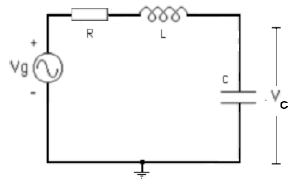
\includegraphics[width=12cm,height=8cm]{Img/pasa-baja}
    
    \vspace{2cm}
    
    \noindent Figura 2. Circuito RLC en serie pasa-alto pasivo\\ 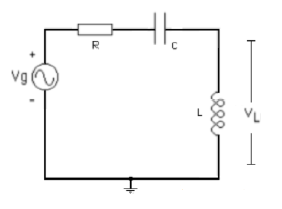
\includegraphics[width=12cm,height=8cm]{Img/pasa-alto}
    
    \vspace{3cm}
    
    \noindent Figura 3. Circuito RLC en serie pasa-banda pasivo\\ 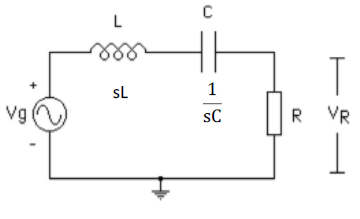
\includegraphics[width=12cm,height=8cm]{Img/pasa-banda}
    
    \vspace{2cm}
    
    \noindent Figura 4. Circuito RLC en serie elimina-banda pasivo\\ 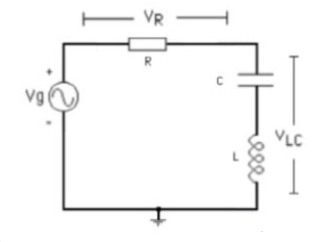
\includegraphics[width=12cm,height=8cm]{Img/elimina-banda}
	
\end{document}